
\chapter{Strategiespiele und Spieltheorie}
\label{cha:Strategiespiele und Spieltheorie}

In den ersten beiden Unterkapiteln werden die Strategiespiele Tic Tac Toe (Abschnitt \ref{sec:Das Strategiespiel Tic Tac Toe}) und Reversi (Abschnitt \ref{sec:Das Strategiespiel Reversi}) vorgestellt und die Regeln dieser beiden Spiele werden festgelegt. Diese beiden Strategiespiele dienen als Umgebungen für den lernenden Agenten (TD-Q Agent). Der TD-Q Agent soll, innerhalb dieser beiden unbekannten Umgebungen, eine möglichst optimale Verhaltensstrategie lernen. \\

Im Unterkapital Spieltheorie (Abschnitt \ref{sec:Spieltheorie}) werden uninformierte Suchbaumverfahren, deren Optimierungsmöglichkeiten, Übergangstabellen und Heuristiken erklärt.\\

Die Minimax-Suche (Abschnitt \ref{subsec:Minimax}) ist ein uninformiertes Suchbaumverfahren. Die Minimax-Suche kann in Zweipersonenstrategiespielen eingesetzt werden, um eine optimale Strategie zu finden. In der Praxis ist das Verfahren jedoch nicht anwendbar. Die Suchbäume realistischer Probleme sind meist entartet bzw. zu groß für eine klassische Minimax-Suche. Die Alpha-Beta-Kürzung (Abschnitt \ref{subsec:Alpha-Beta-Kürzung}) ist eine Verbesserung der Minimax-Suche, dieses Optimierungsverfahren Versucht, den meist viel zu großen Suchbaum zu kürzen, ohne das Endergebnis der Minimax-Suche zu beeinflussen. Wir werden die Minimax-Suche bzw. Alpha-Beta-Suche für die Implementierung des Heuristik Agenten verwenden. Die iterativ vertiefende Tiefensuche (Abschnitt \ref{subsec:Iterativ vertiefende Tiefensuche}) ist ein uninformiertes Suchverfahren, welches Breitensuche und Tiefensuche kombiniert und bis zu einer bestimmten Suchtiefe ein bestmögliches Ergebnis sucht. Wir verwenden die iterativ vertiefende Tiefensuche, für die Verbesserung der vorausschauenden Suche des Heuristik Agenten. \\

Die Übergangstabellen (Abschnitt \ref{subsec:Übergangstabellen}) beschreiben eine Möglichkeit Übergänge zu vermeiden. Übergänge sind identische Spielsituationen, die durch unterschiedliche Aktionssequenzen (eine Folge von Spielzügen) dargestellt werden können, daher scheinen die Spielsituationen unterschiedlich zu sein. Das Zobrist-Hash Verfahren beschreibt eine Möglichkeit die Spielsituationen eindeutig als Zahlwerte darstellen zu können. Wir verwenden dieses Hashverfahren bzw. auch eine Art der Übergangstabellen für das TD-Q lernen. \\

Heuristiken bilden die stärkste Leistungsverbesserung, bezüglich der Rechenzeit, für Suchbaumverfahren. Eine Heuristik (Abschnitt \ref{subsec:Heuristik}) ist eine Bewertungsfunktion B(s), welche für jeden Spielzustand (Stellung der Spielfiguren) s eine Schätzung bereitstellt. Die Schätzung gibt an, wie hoch die Gewinnchance, in einem bestimmten Spielzustand, für den Spielzug ausführenden Spieler, ist. Heuristiken ermöglichen das abbrechen der Suche innerhalb eines Suchbaumes, d.h. auch die nicht Blattkonten des Baumes können Spielergebnisse bereitstellen. Die Kombination von uninformierter Suche und Heuristiken ist nicht mehr uninformiert. Heuristiken stellen zusätzliche Spielinformationen bereit. Die Literatur bezeichnet dies daher als heuristische (informierte) Suche \cite[105]{Ertel}. \\

Wir fassen zusammen: Die Implementierung des Heuristik Agenten erhält eine iterativ vertiefende Alpha-Beta Suche, diese kann auch nicht Blattknoten des Suchbaums, mittels einer Heuristik, bewerten. Wir können also die Rechenzeit des Heuristik Agenten begrenzen, indem wir die maximale Suchtiefe auf 2 Halbzüge begrenzen. Der Heuristik Agent expandiert, wie die iterativ vertiefende Tiefensuche, zu erst alle Knoten in einer Tiefe und erhöht danach schritt für schritt (iterativ) die aktuelle Tiefenschranke, bis zu der maximal möglichen Tiefe. 

\section{Das Strategiespiel Tic Tac Toe}
\label{sec:Das Strategiespiel Tic Tac Toe}

In diesem Abschnitt definieren wir die Regeln des Strategiespiels Tic Tac Toe. Der lernende TD-Q Agent soll für diese Umgebung eine annähernd optimale Strategie lernen. In einem späteren Abschnitt (\ref{subsec:Heuristik} Heuristik) werden wir eine Tic Tac Toe Heuristik für den Heuristik Agenten entwerfen. Wir verwenden Tic Tac Toe als Anwendungsgrundlage für unsere Agentenmodelle verwenden und wir werden die Lernfähigkeit des TD-Q Agenten messen, anhand von Tic Tac Toe Testspielen gegen die anderen beiden Agenten (siehe Abschnitt \ref{cha:Validierung} Validierung). \\
 
Tic Tac Toe ist ein Spiel, welches von genau zwei Spielern gespielt wird. Während eines gesamten Spiels (eine Partie) darf ein Spieler nur Kreuze setzen und der andere Spieler nur Kreise. Wir können uns die Kreuze und Kreise als Spielfiguren vorstellen. Eine Spielfigur die auf das Spielfeld gesetzt wurde, darf seine Position nicht mehr verändern. Das klassische Tic Tac Toe hat 9 Spielfelder (ein 3 x 3 Spielbrett). Innerhalb dieser Arbeit betrachten wir auch ein Tic Tac Toe Spiel mit 16 Spielfeldern (ein 4 x 4 Spielbrett). Der beginnende Spieler muss Kreuzspielfiguren setzen und der nachziehende Spieler Kreisspielfiguren. \\

\paragraph{Spielzüge} jeder Spieler setzt abwechselnd entweder ein Kreuz oder einen Kreis in ein Spielfeld des Spielbretts. Eine Spielfigur kann in jedes freie Spielfeld gesetzt werden, außer dieses ist bereits mit einer anderen Spielfigur besetzt. Die Spieler führen solange ihre Spielzüge aus, bis eine Siegesformation eintritt oder alle Spielfelder besetzt sind. 

\paragraph{Ziel des Spiels} ist es vier Kreuze oder vier Kreise in einer bestimmten Position anzuordnen (Siegesformation). Es existieren mehrere unterschiedliche Anordnungen von Spielfiguren, die das Spiel beenden und einen Sieg herbeiführen. Bei einem 4 x 4 Spielfeld existieren vier vertikale, vier horizontale und zwei diagonale Anordnungen der Spielfiguren, welche einen Sieg herbeiführen würden. Insgesamt zehn verschiedene Siegesanordnungen für beide Spieler. Sind alle Spielfelder besetzt und für keinen der Spieler ist eine Siegesformation aufgetreten, dann gewinnt beziehungsweise verliert keiner der beiden Spieler und es entsteht ein Unentschieden. \\

\begin{figure}[!htbp]
  \centering
  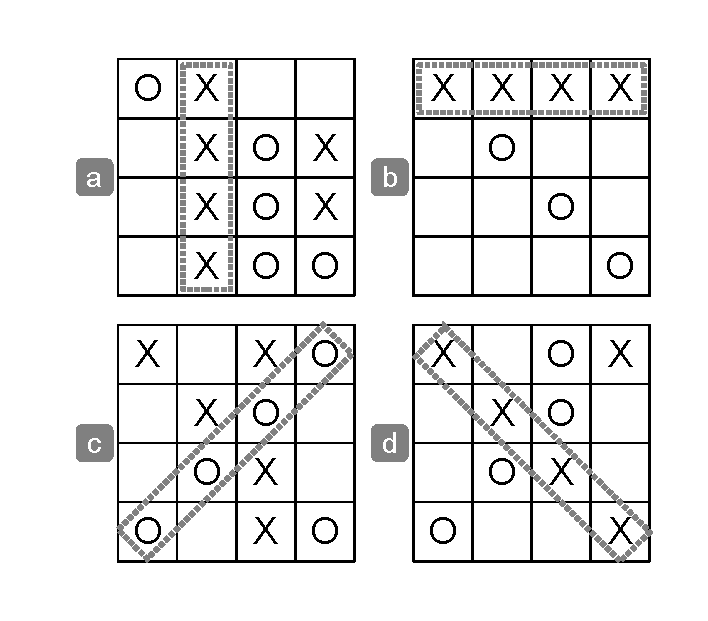
\includegraphics[scale = 0.6]{inhalt/abbildungen/siegesbedingungen_tictactoe.pdf}
  \caption{Tic Tac Toe Siegesformationen.}
  \label{fig:siegesbedingungen_tictactoe}
\end{figure}

Vier mögliche Siegesformationen sind in Abbildung \ref{fig:siegesbedingungen_tictactoe} dargestellt. (a) Kreuz gewinnt, mit einer vertikalen Siegesformation. (b) Kreuz gewinnt, mit einer horizontalen Siegesformation. (c) Kreis gewinnt, mit einer diagonalen Siegesformationen. (d) Kreuz gewinnt, mit einer diagonalen Siegesformation.

\section{Das Strategiespiel Reversi}
\label{sec:Das Strategiespiel Reversi}
In diesem Abschnitt definieren wir die Regeln des Strategiespiels Reversi. Genau wie bei dem Strategiespiel Tic Tac Toe, sollen die Agenten in diesem Spiel gegeneinander antreten und der TD-Q Agent soll eine annähernd optimale Strategie für dieses Spiel lernen. Eine Reversi Heuristik wird ebenfalls in einem späteren Abschnitt entworfen. Reversi ist ein komplexeres Strategiespiel als Tic Tac Toe, d.h. die gelernte Strategie des TD-Q Agenten, benötigt viel mehr Zeit, um eine annähernd optimale Strategie für Reversi zu lernen. Zudem dauert die Berechnung der Stellungsbewertungen, des Heuristik Agenten, (vermutlich) wesentlich länger, als bei Tic Tac Toe. Das Testen der Reversi Heuristik und das Testen der gelernten Reversi Strategie, durch den TD-Q Agenten, könnte viel Rechenzeit beanspruchen. Reversi ist wesentlich komplexer als Tic Tac Toe, weil Reversi 64 Spielfelder (ein 8 x 8 Spielbrett), statt 16 Spielfelder hat. Das Reversi Spielbrett ist um den Faktor 4 größer, als das 4 x 4 Tic Tac Toe Spielbrett. \\

Reversi oder auch Othello genant, ist ein Spiel für zwei Personen die gegeneinander antreten. Eine Person setzt weiße runde Spielsteine und die andere Person schwarze runde Spielsteine. Jede neue Partie Reversie beginnt im selben Ausgangszustand (siehe Abbildung \ref{fig:ausgangssituation_reversi}). Die Spieler setzen nacheinander genau einen Spielstein. Wie beim klassischen Tic Tac Toe behalten die Spieler während des gesamten Spiels ihre Spielsteinfarbe und einmal gesetzte Spielsteine können ihre Position nicht mehr verändern. \\

Anmerkung zu Abbildung \ref{fig:ausgangssituation_reversi}  Die äußeren weiß hinterlegten Reihen, in denen sich Zahlen befinden, dienen dazu, die Positionen der einzelnen Spielfelder genau zu definieren. In der Ausgangsspielsituation befinden sich bereits 2 weiße Spielsteine, an den Positionen (3,4) und (4,3) und zwei schwarze Spielsteine, an den Positionen (3,3) und (4,4). \\

\begin{figure}[!htbp]
  \centering
  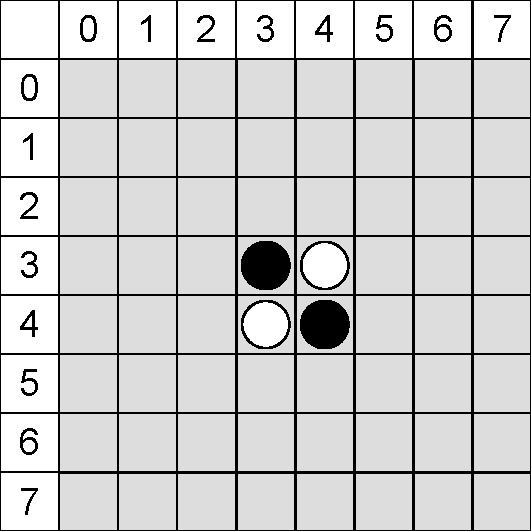
\includegraphics[scale=0.5]{inhalt/abbildungen/ausgangssituation_reversi.pdf}
  \caption{Ausgangsspielzustand Reversi.}
  \label{fig:ausgangssituation_reversi}
\end{figure}



\myparagraph{Spielzüge}
Eine Besonderheit von Reversi ist, dass gesetzte Spielsteine ihre Farbe ändern können. Werden z.B. zwei weiße Spielsteine von zwei schwarzen eingeschlossen, dann werden die weißen Spielsteine in schwarze umgewandelt. Ein korrekter Spielzug muss immer mindestens einen gegnerischen Spielstein erobern. Weiterhin  darf ein Spielstein nur dann gesetzt werden, wenn ein anderer Spielstein (Anker), in einer diagonalen, vertikalen oder horizontalen Linie, existiert. Es dürfen auch keine freien Felder zwischen dem zu setzendem Stein und dem Anker liegen. Ein Anker ist ein Spielstein mit der selben Farbe wie der zu setzende Spielstein. Ein zu setzender Spielstein kann mehrere Anker haben, aber er muss mindestens einen haben.\\

\begin{figure}[!htbp]
  \centering
  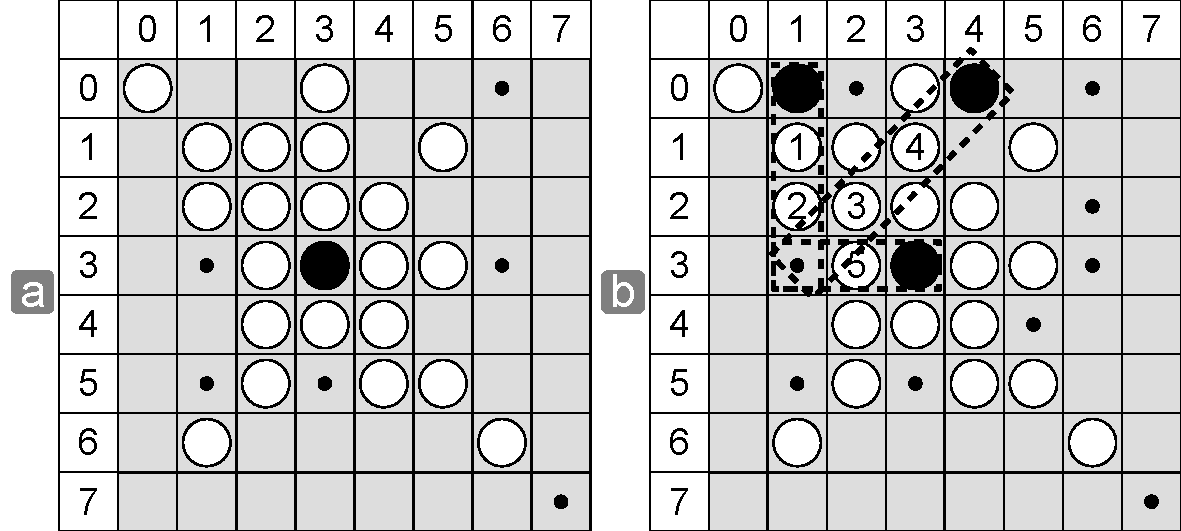
\includegraphics[scale=0.5]{inhalt/abbildungen/zuege_schwarz_reversi.pdf}
  \caption{Spielzugmöglichkeiten Reversi.}
  \label{fig:zuege_schwarz_reversi}
\end{figure}

Anmerkung zu Abbildung \ref{fig:zuege_schwarz_reversi}, diese zeigt zwei möglicherweise nicht in der Praxis auftretende Spielsituationen, die einzig verdeutlichen sollen welche Zugmöglichkeiten der Spieler mit den schwarzen Spielsteinen hat und warum nur diese Züge möglich sind. Die kleinen schwarzen Punkte zeigen die Positionen an denen ein schwarzer Spielstein gesetzt werden darf. (a) Eine Spielsituation mit maximal einem möglichen Anker. (b) Eine Spielsituation mit maximal 3 möglichen Ankern für die Position (3,1). \\

Abbildung \ref{fig:zuege_schwarz_reversi} zeigt zwei verschiedene Reversi Spielsituationen (Schwarz ist am Zug). Die kleinen schwarzen Kreise symbolisieren zulässige Spielzüge. In Spielsituation (a) hat Spieler Schwarz genau 6 Spielzugmöglichkeiten. In jedem dieser Spielzüge erobert er mindestens einen weißen Spielstein und die Reihe wird nicht durch einen schwarzen Spielsein unterbrochen. In Spielsituation (b) hat Spieler Schwarz 9 Spielzugmöglichkeiten. Das setzen eines Spielsteins auf Position (3, 1) würde dem schwarzen Spieler 5 weiße Spielsteine einbringen, da mehrere schwarze Ankersteine diagonal, horizontal und vertikal an diese Position angrenzen.

\paragraph{Ziel des Spiels} ist es, am Ende des Spiels mehr Spielsteine seiner eigenen Farbe zu haben, als der Gegner Spielsteine in seiner Farbe hat. Das Spiel endet, wenn keiner der beiden Spieler mehr einen Spielstein, nach den Regeln des Spiels, auf das Spielbrett setzen kann. \\

\section{Spieltheorie}
\label{sec:Spieltheorie}
In diesem Abschnitt werden wir erklären was uninformierte Suchbaumverfahren, Übergangstabellen und Heuristiken sind. Wir verwenden diese Methoden, aus der Spieltheorie, für die Implementierung unserer Agentenmodelle. Wolfgang Ertel beschreibt Spiele mit Gegenspieler wie folgt \cite[114]{Ertel}: \\ 

Schach, Vier gewinnt, Dame, Tic Tac Toe und Reversi sind strategische Spiele für zwei Personen, die gegeneinander antreten, um nach den Regeln des Spiels, den Gegenspieler zu besiegen. Diese Spiele sind deterministisch, weil das Spiel nicht vom Zufall abhängt und der gleiche Spielzug führt, bei gleichem Ausgangszustand, immer zum selben Spielergebnis. Ein nichtdeterministisches Spiel mit Gegenspieler ist z.B. Backgammon, denn Würfelergebnisse und somit der Zufall sind Bestandteil des Spiels. Die eben genannten Strategiespiele sind alle vollständig beobachtbar (wir verfügen über vollständige Information). Sie sind vollständig überschaubar, weil zu jedem Zeitpunkt des Spiels, das Spielfeld und alle Spielzüge einsehbar sind. Ein nicht vollständig beobachtbares Spiel ist, z.B. Poker oder andere Kartenspiele. Bei einem Poker Spiel sind die gegnerischen Karten und die Karten im Spieldeck unbekannt.\\

''In der künstlichen Intelligenz haben die gebräuchlichsten Spiele in der Regel eine spezielle Natur - die Spieltheoretiker sprechen von deterministischen Zwei-Personen-Nullsummenspielen mit vollständiger Informaiton, bei denen zwei Spieler abwechselt agieren (wie zum Beispiel Schach)\cite[206]{Russell}.'' Die von Russell und Norvig erwähnten Eigenschaften treffen auch auf unsere Strategiespiele zu. Reversi und Tic Tac Toe sind deterministische und vollständig überschaubare Nullsummenspiele, d.h. wir müssen zufällig auftretende Zustandsübergänge und unbekannte Informationen, in unseren Heuristiken und Lernverfahren, nicht berücksichtigen. Nullsummenspiel bedeutet: gewinnt ein Spieler eine Partie, dann verliert der Gegenspieler automatisch in gleicher Höhe.

\subsection{Minimax-Suche}
\label{subsec:Minimax}
Wir werden die von Russell und Norvig beschriebene Minimax-Suche, für die Implementierung des vorausschauenden Heuristik Agenten verwenden, daher werden wir die Minimax-Suche genauer erklären. \\

''In einem normalen Suchproblem wäre die optimale Lösung eine Folge von Aktionen die zu einem Zielzustand führt - einem Endzustand, bei dem es sich um einen Gewinn handelt. In einer adversialen Suche dagegen hat Min auch noch etwas zu sagen. Max muss also eine mögliche Strategie finden, die den Zug von Max ab dem Ausgangszustand angibt und dann die Züge von Max in den Zuständen, die aus den einzelnen Gengenzügen von Min auf diese Züge resultieren usw \cite[208]{Russell}.''

Anders ausgedrückt, berücksichtigt die Minimax-Suche, gegenüber anderen uninformierten Suchverfahren (z.B. Breitensuche oder Tiefensuche), dass ein Gegenspieler existiert. Der Gegenspieler führt den für sich optimalen Zug aus, d.h. er wird den anderen Spieler, wann immer es geht, behindern. Ein Spieler wird als MAX bezeichnet und der Gegenspieler als MIN. Spieler MAX versucht einen maximalen Gewinn für sich zu erlangen und Spieler MIN versucht den erreichbaren Gewinn von MAX zu minimieren.\\

In Abbildung \ref{fig:minimax_tictactoe} wird der Ablauf der Minimax-Suche veranschaulicht. Der Minimax-Suchbaum berücksichtigt jeden Zustand indem sich die Spielwelt befinden kann. Im ersten Spielzug könnte Spieler MAX sein Kreuzspielstein in die obere linke Ecke setzen, daraus ergeben sich neue Zustandsmöglichkeiten. Spieler MIN könnte seinen Kreisspielstein ein Feld weiter rechts und in die selbe Reihe wie Spieler MAX setzen. Die Abbildung bzw. die Minimax-Suche muss rekursiv betrachtet werden, denn erst in den Blattknoten des Suchbaums, sind die Spielergebnisse zu finden. Von seinen Blattknoten ausgehend entscheidet sich MIN für den geringsten Nutzwert und MAX für den höchsten Nutzwert. Die Entscheidungen stehen in direkter Abhängigkeit zur vorherigen Entscheidung des Gegenspielers. \\
  
\begin{figure}[!htbp]
  \centering
  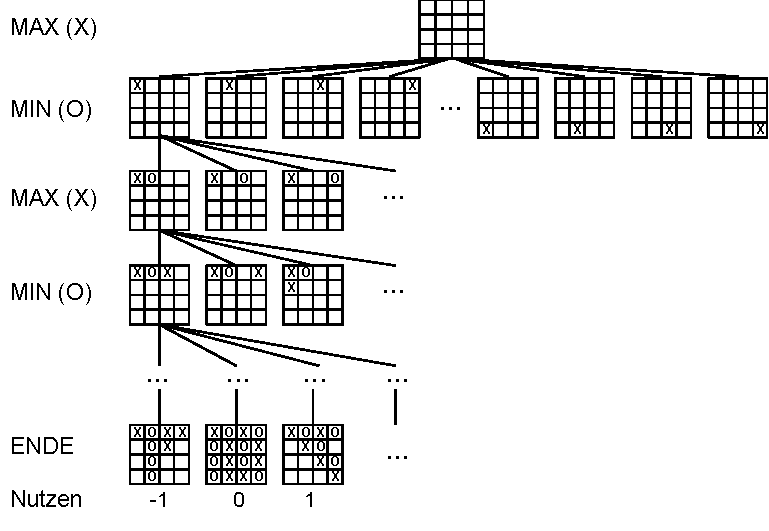
\includegraphics{inhalt/abbildungen/minimax_tictactoe.pdf}
  \caption{Ein (partieller) Suchbaum vgl. \cite[208]{Russell}}
  \label{fig:minimax_tictactoe}
\end{figure} 

''Der effektive Verzweigungsfaktor beim Schachspiel liegt etwa bei 30 bis 35. Bei einem typischen Spiel mit 50 Zügen pro Spieler hat der Suchbaum dann mehr als $30^{100} \approx 10^{148}$ Blattknoten. Der Suchbaum lässt sich also bei weitem nicht vollständig explorieren. Hinzu kommt, dass beim Schachspiel oft mit Zeitbeschränkung gespielt wird. Wegen dieser Realzeitanforderung wird die Tiefe des Suchbaums auf eine passende Tiefe, zum Beispiel acht Halbzüge, beschränkt \cite[114 \psq]{Ertel}.''

Wolfgang Ertel beschreibt in diesem Zitat das Verhältnis von Problemkomplexität und Suchbaumgröße. Genau dieses Problem wird auch das TD-Q-Lernen stark beeinflussen. Das TD-Q-Lernen exploriert zwar keinen Suchbaum, jedoch steigen die nötigen Lerndurchläufe, bis zur Konvergenz zu einer optimalen Strategie, exponentiell mit der Komplexität des Problems. Wir werden im Kapitel Validierung praktisch zeigen, welche Auswirkungen verschieden komplexe Probleme, auf das TD-Q-Lernen, haben. Im Kapitel Auswertung werden wir mögliche Lösungsmöglichkeiten vorstellen.

\subsection{Alpha-Beta-Kürzung}
\label{subsec:Alpha-Beta-Kürzung}
Im vorherigen Abschnitt haben wir erklärt was genau die Minimax-Suche ist und warum diese praktisch nicht anwendbar ist (siehe \cite[114 \psq]{Ertel}). Eine Möglichkeit die Rechenzeit der Minimax-Suche zu verbessern, ist das Kürzen oder Beschneiden des Suchbaums(eng. Pruning). Wir verwenden diese Minimax-Optimierung für die Implementierung eines vorausschauenden Heuristik Agenten.

Wolfgang Ertel erklärt die Alpha-Beta Suche wie folgt vgl. \cite[116]{Ertel}:
Beim Alpha-Beta-Kürzen wird der Teil des Suchbaums beschnitten, der keinen Effekt auf das Ergebnis der Minimax Suche hat. Der Minimax Algorithmus wird um zwei Parameter Alpha und Beta ergänzt. Die Bewertung erfolgt an jedem Blattknoten des Suchbaums. Alpha enthält den aktuell größten Wert, für jeden Maximum Knoten, der bisher bei der Traversierung (Erkundung oder das Durchlaufen) des Suchbaums gefunden wurde. In Beta wird für jeden Minimum Knoten der bisher kleinste gefundene Wert gespeichert. Ist Beta an einem Minimum Knoten kleiner oder gleich Alpha ($Beta \leq Alpha$), so kann die Suche unterhalb von diesem Minimum Knoten abgebrochen werden. Ist Alpha an einem Maximum Knoten größer oder gleich Beta ($Alpha \geq Beta$), so kann die Suche unterhalb von diesem Maximum Knoten abgebrochen werden. \\

\begin{figure}[!htbp]
  \centering
  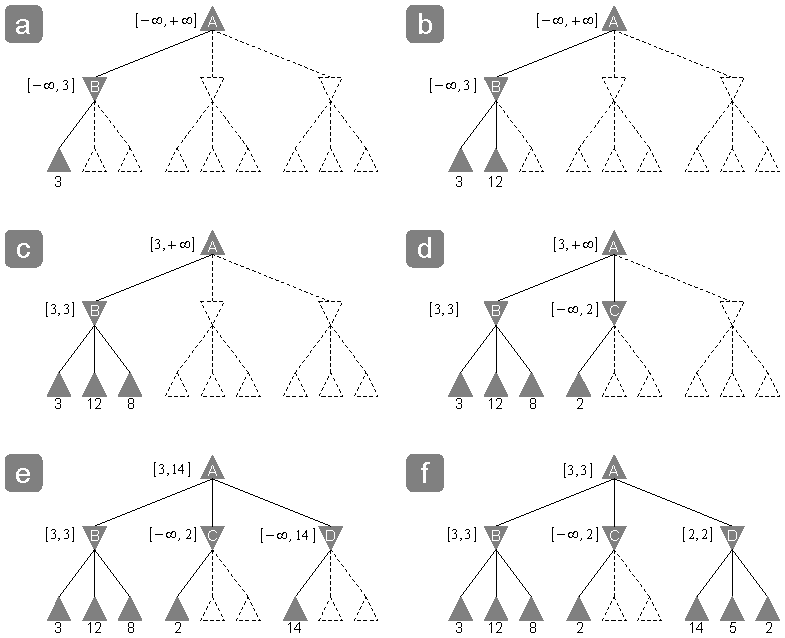
\includegraphics[scale = 0.8]{inhalt/abbildungen/alpha_beta_suchbaum.pdf}
  \caption{Ein Alpha Beta Suchbaum \cite[213]{Russell}.}
  \label{fig:minimax_tictactoe}
\end{figure} 

Verdeutlichen wir das Alpha-Beta-Pruning an Hand eines Beispiels (Abbildung \ref{fig:minimax_tictactoe}). Ein Dreieck mit der Spitze nach oben ist ein Maximumknoten und ein Dreieck mit der Spitze nach unten ist ein Minimumknoten. Leere Dreiecke ohne einen bezeichnenden Buchstaben und gestrichelter Umrandung sind noch nicht explorierte Knoten. Durchgängige Linien verweisen auf bereits besuchte Pfade und gestrichelte Linien verweisen auf noch nicht besuchte Pfade. Die Zahlen unterhalb der Blattknoten sind die Nutzwerte die der maximierende Spieler erhält, wenn er den Pfad bis zu diesem Blattknoten durchschreitet. \\

(a) Minimum Knoten B findet einen Nutzwert 3, da dieser Wert der bisher kleinste gefundene Wert ist wird er in Beta gespeichert. \\

(b) Der Minimum Knoten B exploriert einen zweiten möglichen Nutzwert 12. Dieser Wert ist höher als der vorher gefundene und in Beta gespeicherte Wert 3, daher wird der minimierende Spieler versuchen diesen Nutzwert für den maximierenden Spieler zu vermeiden. Der neue Wert wird vom Minimum Knoten B ignoriert und Beta bleibt unverändert. \\

(c) Minimum Knoten B findet den Wert 8, dieser ist genau wie 12 größer als 3 und daher wird Spieler MIN vermeiden, dass Spieler MAX zu diesem Spielergebnis gelangt. Minimum Knoten B hat alle seine nachfolgenden Knoten exploriert. Maximum Knoten A wird vom Minimum Knoten B maximal den Nutzwert 3 erhalten, somit ergibt sich für den Maximum Knoten A, dass dieser mindestens den Nutzwert 3 erreichen kann. \\

(d) Ein weiterer Minimum Knoten ist C. Der erste Blattknoten von C liefert einen Nutzwert von 2, weil dieser Wert der erste gefundene Wert unterhalb des Minimum Knotens C ist, wird er in Beta gespeichert. C wird Maximum Knoten A maximal einen Nutzwert 2 liefern. A wiederum kann durch Minimum Knoten B bereits einen minimalen Nutzwert von 3 erhalten und hat diesen in Alpha gespeichert. Es gilt $Beta \leq Alpha$ und es ist nicht notwendig die Knoten unterhalb von C weiter zu explorieren. Selbst wenn ein größerer Nutzwert gefunden werden würde, entscheidet sich der minimierende Spieler trotzdem für den kleineren Wert und würde ein kleinerer Nutzwert als 2 gefunden werden, dann entscheidet sich der maximierende Spieler für den Nutzwert 3, den Minimum Knoten B liefert. Folglich kann der Suchbaum an dieser Stelle abgeschnitten werden, weil weitere gefundene Nutzwerte keinen Einfluss mehr auf das Ergebnis haben. \\

(e) Der letzte von A zu erreichende Minimum Knoten wird exploriert. Der erste Blattknoten unterhalb des Minimum Knoten D liefert den Nutzwert 14. Dieser Wert wäre für Maximum Knoten A eine starke Verbesserung, weil dieser bisher nur maximal einen Nutzwert von 3 erreichen konnte. Der minimierende Spieler hat noch zwei weitere Möglichkeiten(Knoten) zu explorieren und daher wird er versuchen einen geringeren Nutzwert als 14 zu finden. \\

(f) Minimum Knoten D findet in den beiden letzten Blattknoten die Nutzwerte 5 und 2. Der minimierende Spieler wählt die Möglichkeit mit dem geringsten Nutzwert 2. Dieser Nutzwert wird zum neuen Beta Wert. Der Suchbaum wird unterhalb vom Minimum Knoten D jedoch nicht abgeschnitten, weil der Nutzwert 2 erst im zuletzt explorierten Knoten gefunden wurde. Theoretisch könnten zwei Pfade unterhalb des Minimum Knoten D abgeschnitten werden, wenn der Blattknoten mit dem Nutzwert 2 zuerst exploriert worden wäre.

Praktisch ist die Alpha-Beta Kürzung ebenfalls nicht anwendbar. Selbst wenn ein großer Teil des Suchbaums abgeschnitten werden kann, ohne das Ergebnis zu beeinflussen, dann ist eine Exploration des Suchbaums immer noch, aus Gründen zu großer Rechenzeit, zu teuer. Wir werden daher noch die iterativ vertiefende Tiefensuche und Heuristiken behandeln. 

\subsection{Iterativ vertiefende Tiefensuche}
\label{subsec:Iterativ vertiefende Tiefensuche}
Um dieses Verfahren zu beschreiben, fassen wir die Ausführungen, zum Thema iterativ vertiefende Tiefensuche, von Russell und Norvig vgl. \cite[116]{Russell} zusammen:\\

Die iterativ vertiefende Tiefensuche (eng. Iterative Deepening) ist ein kombinatorisches bzw. uninformiertes Suchbaumverfahren und kombiniert die Breitensuche mit der Tiefensuche. Die Strategien der uninformierten Suchverfahren haben keine zusätzlichen Informationen über Zustände, außer den in der Problemdefinition vorgegebenen. Alles was sie tun können, ist, Nachfolger zu erzeugen und einen Zielzustand von einem Nichtzielzustand zu unterscheiden. Die Reihenfolge der Suche ist entscheidend für die Unterscheidung der einzelnen uninformierten Suchverfahren. \\
 
Die Breitensuche expandiert (erweitert oder vergrößert) zu erst alle Nachfolger (Knoten eines Suchbaums) die in derselben Tiefe liegen, beginnend mit dem Wurzelknoten. Sind alle Nachfolger einer Tiefe expandiert, dann werden deren Nachfolger nacheinander expandiert. Diesen Schritt wiederholt die Breitensuche bis ein gesuchtes Ergebnis gefunden wird oder der Suchbaum vollständig exploriert (erkundet) ist. \\

Die Tiefensuche expandiert zuerst die tiefsten Knoten des Suchbaums(Depth-first). Erreicht die Tiefensuche einen Endknoten der nicht dem gesuchten Ergebnis entspricht, dann werden die alternativen Knoten des letzten expandierten Knotens, der sich eine Tiefenebene höher befindet, expandiert. \\

Kombinieren wir diese beiden uninformierten Suchverfahren miteinander und mit einer Grenze für die Suchtiefe, erhalten wir die iterative Tiefensuche. Diese expandiert zuerst die Nachfolger des Wurzelknotens der Suchtiefe 1. Sind alle Knoten auf dieser Ebene expandiert, dann wird die Schranke für die aktuelle Suchtiefe um 1 erhöht (Iteration) und die Knoten der Suchtiefe 2 werden expandiert. Diese Schritte wiederholt die Tiefensuche bis ein Ziel gefunden wird. \\  

Für diese Arbeit ist dieses Verfahren relevant, weil der vorausschauende Heuristik Agent bzw. die in seiner Implementierung realisierte Alpha-Beta Suche, an die iterativ vertiefende Tiefensuche angepasst wird. Der Agent wird also nicht den gesamten Zustandsraum (Suchbaum) durchsuchen, sondern seine Zugvorausschau wird auf eine bestimmte Anzahl von Zügen begrenzt werden. Meistens wird eine Zugvorausschau von 2 Zügen nicht ausreichen, um einen Blattknoten des Suchbaumes zu erreichen, daher führen wir noch Heuristiken (Bewertungsfunktionen) ein.\\

\subsection{Übergangstabellen}
\label{subsec:Übergangstabellen}
Eine Übergangstabelle (eng. transition table) ist eine Tabelle in der Spielsituationen mit verschiedenen Attributen gespeichert werden (vgl. \cite[215\psq]{Russell}). Übergänge sind der Grund dafür, dass der gleiche Spielzustand durch unterschiedliche Spielzugsequenzen auftritt (siehe Abbildung \ref{fig:transitionen_tictactoe}). \\

\begin{figure}[!htbp]
  \centering
  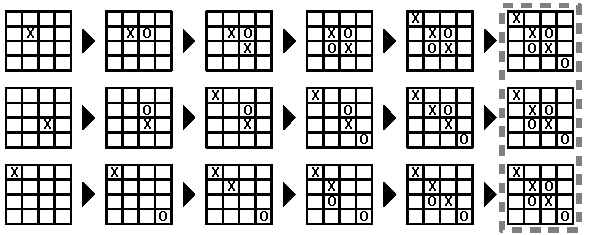
\includegraphics{inhalt/abbildungen/transitionen_tictactoe.pdf}
  \caption{Verschiedene Spielzugsequenzen enden im selben Spielzustand.}
  \label{fig:transitionen_tictactoe}
\end{figure} 

Übergänge innerhalb des Suchbaums verursachen Redundanzen. Für jede dieser Redundanzen wird eine erneute Suche durchgeführt, falls diese nicht durch Alpha-Beta-Kürzung abgeschnitten werden. Sollten diese Übergänge vermieden werden können, dann würde sich die Rechenzeit der Suchverfahren weiter verringern, weil weniger Spielzustände durchsucht bzw. expandiert werden müssen. \\

Wir können uns das TD-Q-Lernen, als eine Art Übergangstabelle vorstellen. Die Tabelle würde 3 Spalten haben. Die erste Spalte beinhaltet den Spielzustand, die zweite Spalte die dazugehörige Aktion und die dritte Spalte enthält den Q-Wert (Nutzwert), d.h. Zustand/Aktionspaare werden auf Q-Werte abgebildet. Diese Tabelle wird nicht unbedingt geführt um Redundanzen zu vermeiden, sondern eher um Nutzeninformationen zu speichern.

\myparagraph{Zobrist Hash}
''Wenn ein Computerprogramm einen Gegenstand in einer großen Tabelle speichert, muss die Tabelle zwangsläufig durchsucht werden, um den Gegenstand wiederzuverwenden bzw. zu referenzieren. Dies gilt solange, bis eine Tabellendresse aus dem Gegenstand selbst, in systematischer weise, berechnet werden kann. Eine Funktion die Gegenstände in Adressen umwandelt ist ein Hash-Algorithmus, und die daraus resultierende Tabelle ist eine Hashtabelle \cite[3]{Zobrist}.'' \\

Zobrist-Hashing ermöglicht es, Spielzustände eindeutig als Zahlenwerte zu definieren. Berechnen wir den Zobrist-Hash eines Spielzustandes, dann ist dieser immer gleich, selbst wenn der Spielzustand durch verschiedene Aktionssequenzen repräsentiert werden kann. Das Zobrist-Hashverfahren ist sehr wichtig für unseren TD-Q lernenden Agenten, weil die Spielsituationen, als Zobrist-Hash, in der Q-Wertetabelle eingetragen werden können.

\begin{figure}[!htbp]
  \centering
  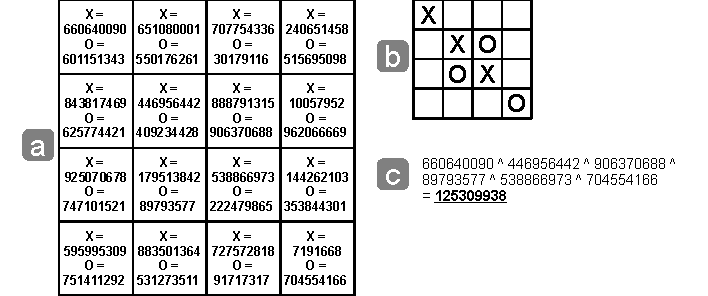
\includegraphics[scale = 1.3]{inhalt/abbildungen/zobrist_hash_tictactoe.pdf}
  \caption{Zobrist Hashing von Spielzuständen.}
  \label{fig:zobrist_hash_tictactoe}
\end{figure} 


In Abbildung \ref{fig:zobrist_hash_tictactoe} wird das Zobrist Hash Verfahren auf den redundanten Spielzustand aus Abbildung \ref{fig:transitionen_tictactoe} angewendet. Schritt 1: (a) wir weisen jedem Spielfeld zwei zufällige ganzzahlige Werte zu im Bereich von 0 bis maximal $1 \times 10^{9}$. Einen zufälligen Wert für den Kreuzspielstein an dieser Position und einen für den Kreisspielstein. Das 4x4 Tic Tac Toe Spielbrett sollte insgesamt 32 verschiedene Werte erhalten. Spielsituation (b) soll in einen Zobrist-Hash umgewandelt werden. \\

Der Zobrist-Hash berechnet sich wie folgt (c), ist die aktuelle Position mit einem Kreuzspielstein oder einem Kreisspielstein besetzt, dann wähle den entsprechenden Wert aus der Werttabelle (a). Dies wiederhole für jedes besetzte Spielfeld. Wir verknüpfen die bestimmten Werte, mittels eines exklusiven bzw. bitweisen Oder (XOR). Das Ergebnis ist eine Adresse die exakt den Spielzustand (b) referenziert. \\

\subsection{Heuristik}
\label{subsec:Heuristik}
''Heuristiken sind Problemlösungsstrategien, din in vielen Fällen zu einer schnelleren Lösung führen als die uninformierte Suche. Es gibt jedoch keine Garantie hierfür. Die heuristische Suche kann auch viel mehr Rechenzeit beanspruchen und letztlich dazu führen, dass die Lösung nicht gefunden wird \cite[105]{Ertel}.''\\

Wir leiten aus der Definition von Wolfgang Ertel folgendes ab:\\ 
Eine Heuristik oder Bewertungsfunktion berechnet eine Gewinnchance für einen gegebenen Spielzustand, d.h. ob der Spieler in diesem Spielzustand eher gewinnen oder verlieren könnte. Die Verwendung einer Heuristik ist keine Garantie für ein korrektes Ergebnis. In der Regel, wird für bessere Rechenzeit, ein mögliches schlechteres Ergebnis akzeptiert, d.h. eine heuristische Zustandsbewertung, muss nicht dem wahren Nutzen des Zustands entsprechen. Die Qualität einer Heuristik ist demnach ausschlaggebend für das Spielergebnis. Ein schlechte Stellungsbewertung (Heuristik), kann schlechte Spielzüge verursachen oder fatale Spielzüge des Gegners übersehen. \\

Die Verwendung einer Heuristik ermöglicht es, nicht Blattknoten eines Spielbaumes zu bewerten, somit können Suchverfahren die Suche in einer bestimmten Tiefe abbrechen und das bisher beste bisher gefundene Ergebnis zurückliefern. Aus Gründen der starken Rechenzeitverbesserung implementieren wir Heuristiken für den nicht lernenden Agenten. \\

Eine Bewertungsfunktion B(s) für ein Schachspiel enthält folgende Elemente, wobei s der Parameter für den Spielzustand ist\cite[119]{Ertel}: \\

B(s) = $a_1$ x Material +  $a_2$ x Bauernstruktur + $a_3$ x Königssicherheit \\
\tab \tab + $a_4$ x Springer im Zentrum + $a_5$ x Läufer Diagonalabdeckung + ..., \\ 

das mit Abstand wichtigste Feature (Merkmal) "Material" nach der Formel \\

\tab \tab Material = Material(eigenes Team) - Material(Gegner) \\

Material(Team) = Anzahl Bauern(Team) x 100 + Anzahl Springer(Team) x 300 \\
\tab \tab \tab + Anzahl Läufer(Team) x 300 + Anzahl Türme(Team) x 500 \\
\tab \tab \tab + Anzahl Damen(Team) x 900 \\

Wolfgang Ertel schreibt sinngemäß \cite[118]{Ertel}:
Diese Schach Heuristik ist entstanden aus der Zusammenarbeit von Schachexperten und Wissensingenieuren. Die Schachexperten verfügen über Wissen und Erfahrungen bezüglich des Schachspiels, der Strategien, guter Zugstellungen und schlechter Zugstellungen. Der Wissensingenieur hat die meist sehr schwierige Aufgabe dieses Wissen in eine, für ein Programm, anwendbare Form zu bringen. \\

Formal definieren Russell und Norvig Bewertungsfunktionen \cite[218]{Russell}: 

\begin{equation*}
\hat{U}_\theta(s) = \theta_1 f_1(s) + \theta_2 f_2(s) + ... + \theta_n f_n(s),
\end{equation*}

als eine gewichtete Lineare Funktion einer Menge von Merkmalen (oder Basisfunktionen) $f_1, ..., f_n$. Die Parameter $\theta = \theta_1, ... \theta_n$ sind die Gewichtungen der einzelnen Merkmale, d.h. ein Parameter bestimmt, wie ''wichtig'' ein Merkmal ist.

\myparagraph{Tic Tac Toe Heuristik}
Für eine bessere Beschreibung der Tic Tac Toe Heuristik, werden wir eine konkrete Identifikation der einzelnen Spielfelder vornehmen. In Abbildung \ref{fig:tictactoe_spielfeld_indizes} weisen wir jedem der Spielfelder einen Index zu. Die Eckfelder (0,0), (0,3), (3,0) und (3,3) sind weiß. Die Randfelder (1,0), (2,0), (0,1), (0,2), (3,1), (3,2), (1,3) und (2,3) sind grau. Die Mittelfelder (1,1), (1,2), (2,1) und (2,2) sind schwarz. \\

\begin{figure}[!htbp]
  \centering
  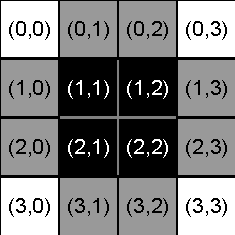
\includegraphics[scale = 0.7]{inhalt/abbildungen/tictactoe_spielfeld_indizes.pdf}
  \caption{Die Indizes der einzelnen Spielfelder.}
  \label{fig:tictactoe_spielfeld_indizes}
\end{figure}

Das erste Merkmal unserer Tic Tac Toe Heuristik ist, die Kontrolle der mittleren Spielfelder, d.h. Spielsituationen in denen die mittleren Spielfelder mit eigenen Spielfiguren besetzt sind, erhalten eine höhere Bewertung. Die Kontrolle des mittleren Spielfeldes bezeichnet ein Eröffnungsmerkmal. Die erste Spielfigur, soll in die mittleren Spielfelder gesetzt werden und die zweite eigene Spielfigur, soll in die vom Gegenspieler nicht gestörte mittlere Position gesetzt werden. \\

\begin{figure}[!htbp]
  \centering
  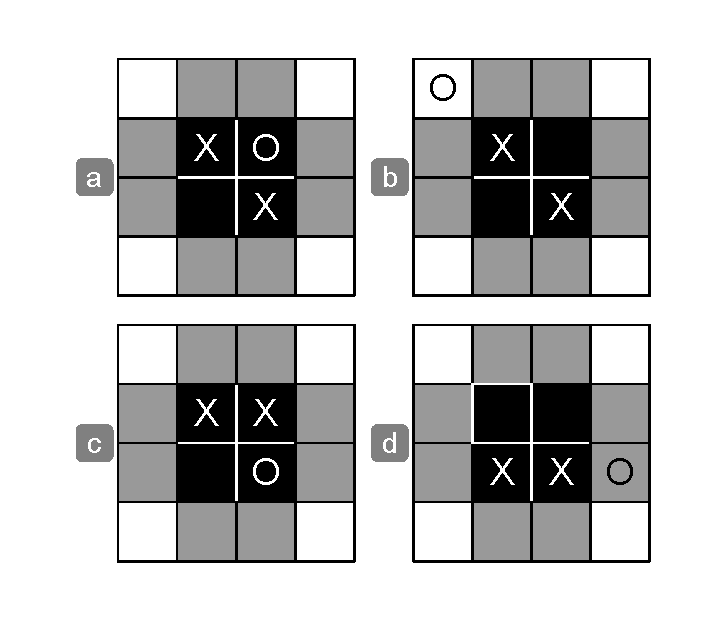
\includegraphics[scale = 0.7]{inhalt/abbildungen/tictactoe_mid_control.pdf}
  \caption{Tic Tac Toe Eröffnungssituationen.}
  \label{fig:tictactoe_mid_control}
\end{figure}

\begin{figure}[!htbp]
  \centering
  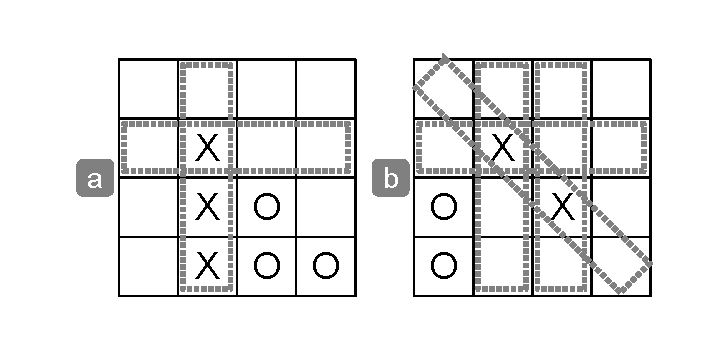
\includegraphics[scale = 0.7]{inhalt/abbildungen/tictactoe_formations.pdf}
  \caption{Tic Tac Toe Formationsmöglichkeiten.}
  \label{fig:tictactoe_formations}
\end{figure}



Das zweite Merkmal der Tic Tac Toe Heuristik ist, die Beachtung der ungestörten Möglichkeiten für Siegesformationen. Eine Formationsmöglichkeit wird gefährlicher bzw. attraktiver, je mehr gleiche Spielfiguren sich bereits in dieser befinden. Wir stellen bei diesem Merkmal gegenüber: wie viele, vom Gegenspieler nicht gestörte, Formationsmöglichkeiten  einem Spieler zur Verfügung stehen und wie viele ungestörte Formationsmöglichkeiten der Gegenspieler hat. 


\myparagraph{Reversi Heuristik}
%http://www.samsoft.org.uk/reversi/strategy.htm
\begin{figure}[!htbp]
  \centering
  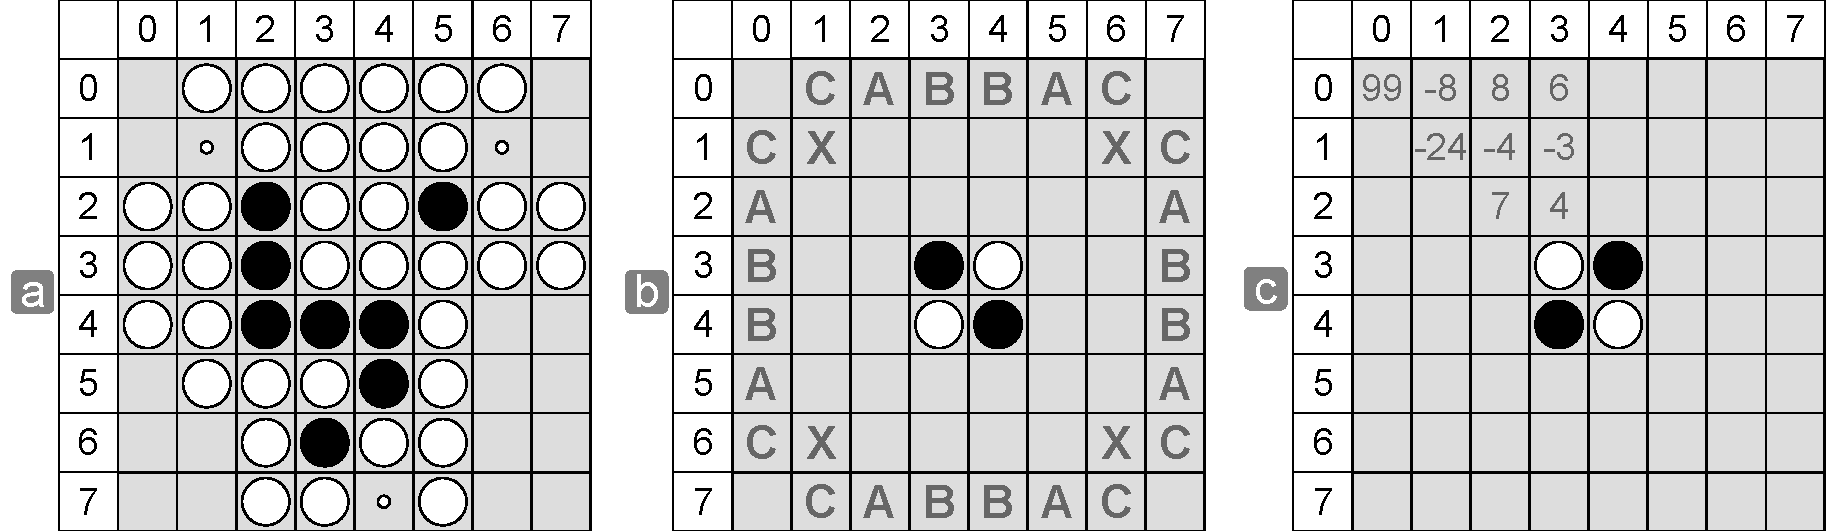
\includegraphics[scale = 0.5]{inhalt/abbildungen/reversi_movement_notation_positioning.pdf}
  \caption{Merkmale einer Reversi Heuristik.}
  \label{fig:reversi_movement_notation_positioning}
\end{figure}
